\section{Processor Equivalence}
In this section, we will discuss the power equivalence problem.
\\
I will present the closed-form equal formula about the load from three different kind of injection position,load from corner,boundary and inner grid position in regular mesh.
\\
In addition, considering the unit core with or without the front-end processor,the data transportation schema can be considered as two situation with front-end  and without front-end transportation.

\vspace*{5pt}

For a homogeneous regular mesh, which can be collapsed into an equivalent node, the notation is presented as follows.\\

\begin{itemize}

\item $\alpha_{0}$: The load fraction assigned to the root processor.
\item $\alpha_{i}$: The load fraction assigned to the $i$th processor.
\item $\omega_{i}$: The inverse computing speed on the $i$th processor.
\item $\omega_{eq}$: The inverse computing speed on an equivalent node collapsed from a regular mesh.
\item $z_{i}$: The inverse link speed on the $i$th link.
\item $T_{cp}$: Computing intensity constant.The entire load can be transmitted in $z_{i}T_{cp}$ on the $i$th processor.
\item $T_{cm}$: Communication intensity constant.The entire load can be transmitted in $z_{i}T_{cm}$ seconds over the $i$th link.
\item $T_{f,m}$: The finish time of the whole regular network.Here $T_{f,m}$ is equal to $\omega_{eq}T_{cp}$.
\item $T_{f,0}$: The finish time for the entire divisible load solved on the root processor.Here $T_{f,0}$ is equal to $1 \times \omega_{0}T_{cp}$, that is $\omega_{0}T_{cp}$.

\end{itemize}
\vspace*{5pt}
\subsection{With Front-end Schema}
\vspace*{5pt}
I investigate the simple case first and then deduce the more general closed form formula for the homogeneous regular mesh situation.
\vspace*{5pt}

\subsubsection{Load From Corner}
\begin{itemize}
\vspace*{5pt}
\item 2*2 regular mesh Fig.\ref{22f}
\item 2*3 regular mesh Fig.\ref{23f}
\item 2*n regular mesh,for example $n = 10$ Fig.\ref{210f}
\item 3*n regular mesh,for example $n = 8$ Fig.\ref{38f}
\item m*n regular mesh,for example $m = 5, n = 5$ Fig.\ref{410f}
\end{itemize}

According to Fig.\ref{22f},data injection position comes from corner.

There are four unit cores to handle the whole workload in the regular mesh.

\begin{figure}[h]
\centering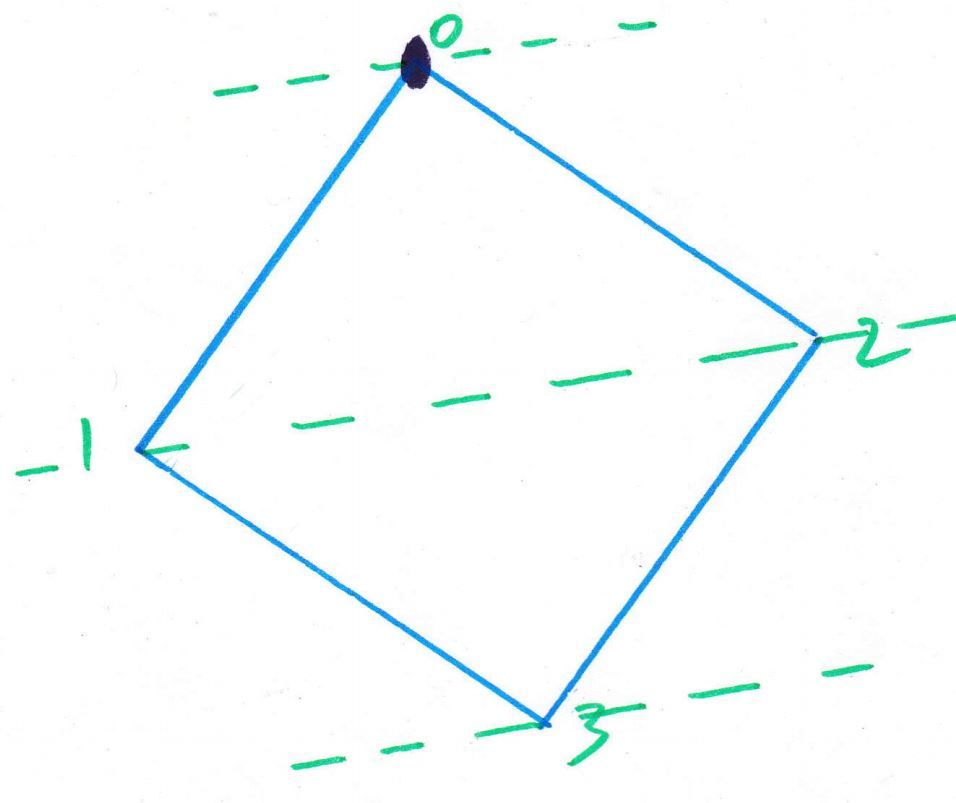
\includegraphics[width = 0.7\linewidth]{figure/c22_f}
\caption{2*2 regular mesh}
\label{22f}
\end{figure}


$$\alpha_{0} \omega T_{cp} = T_{f,m}$$ 
$$\alpha_{1} \omega T_{cp} = T_{f,m}$$
$$\alpha_{2} \omega T_{cp} = T_{f,m}$$
$$\alpha_{1}zT_{cm} + \alpha_{3}\omega T_{cp} = T_{f,m}$$
$$\sigma = \frac{zT_{cm}}{\omega T_{cp}}$$


\begin{equation}
{
\left[ \begin{array}{ccc}
1 & 2 & 1\\
1 & -1 & 0\\
0 & \sigma-1 & 1
\end{array} 
\right ]} \times \left[ \begin{array}{c}
\alpha_{0} \\
\alpha_{1} \\
\alpha_{3} 
\end{array} 
\right ] = \left[ \begin{array}{c}
1 \\
0 \\
0 
\end{array} 
\right ]
\end{equation}

\vspace*{50pt}
According to Fig.\ref{23f}, the data load injection comes from corner and there are
six cores to handle the whole workload.

\begin{figure}[h]
\centering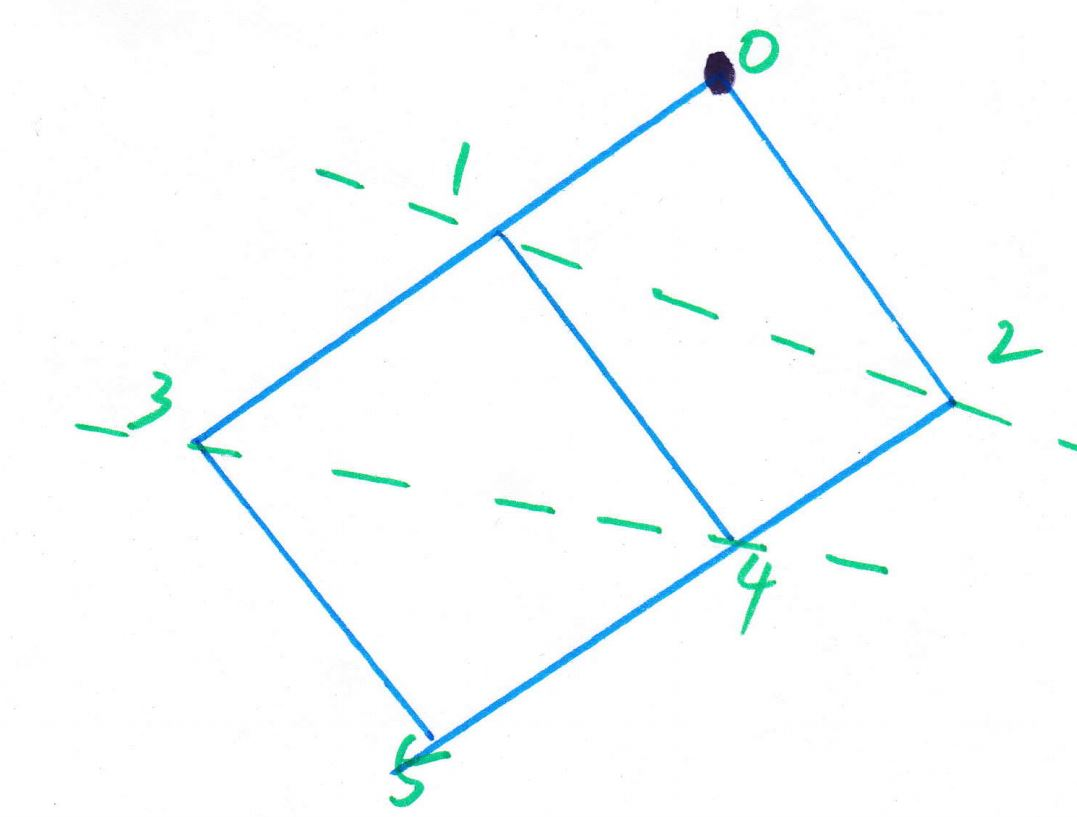
\includegraphics[width=0.7\linewidth]{figure/c23_f}
\caption{2*3 regular mesh}
\label{23f}
\end{figure}

$$\alpha_{0} \omega T_{cp} = T_{f,m}$$ 
$$\alpha_{1} \omega T_{cp} = T_{f,m}$$
$$\alpha_{2} \omega T_{cp} = T_{f,m}$$
$$\alpha_{1}zT_{cm} + \alpha_{3}\omega T_{cp} = T_{f,m}$$
$$\alpha_{2}zT_{cm} + \alpha_{4}\omega T_{cp} = T_{f,m}$$
$$(\alpha_{1} + \alpha_{3})zT_{cm} + \alpha_{5}\omega T_{cp} = T_{f,m}$$

$$\sigma = \frac{zT_{cm}}{\omega T_{cp}}$$
\begin{equation}
{
\left[ \begin{array}{cccc}
1 & 2 & 2 & 1\\
1 & -1 & 0 & 0\\
0 & \sigma-1 & 1 & 0\\
0 & \sigma-1 & \sigma & 1
\end{array} 
\right ]} \times \left[ \begin{array}{c}
\alpha_{0} \\
\alpha_{1} \\
\alpha_{3} \\
\alpha_{5}
\end{array} 
\right ] = \left[ \begin{array}{c}
1 \\
0 \\
0 \\
0
\end{array} 
\right ]
\end{equation}

\vspace*{50pt}

Considering the $2*n$ situation, the formula is:


$$\alpha_{0} \omega T_{cp} = T_{f,m}$$ 
$$\alpha_{1} \omega T_{cp} = T_{f,m}$$
$$\alpha_{2} \omega T_{cp} = T_{f,m}$$
$$\alpha_{1}zT_{cm} + \alpha_{3}\omega T_{cp} = T_{f,m}$$
$$\alpha_{2}zT_{cm} + \alpha_{4}\omega T_{cp} = T_{f,m}$$
$$(\alpha_{1} + \alpha_{3})zT_{cm} + \alpha_{5}\omega T_{cp} = T_{f,m}$$
$$\vdots$$
$$(\alpha_{1} + \alpha_{3} +\cdots + \alpha_{2 \times n - 1})zT_{cm} +\alpha_{2 \times n + 1} \omega T_{cp} = T_{f,m}$$
$$\sigma = \frac{zT_{cm}}{\omega T_{cp}}$$

\vspace*{50pt}
For example, the $n = 10$ Fig. \ref{210f}, the formula as follows:

\begin{figure}[h]
\centering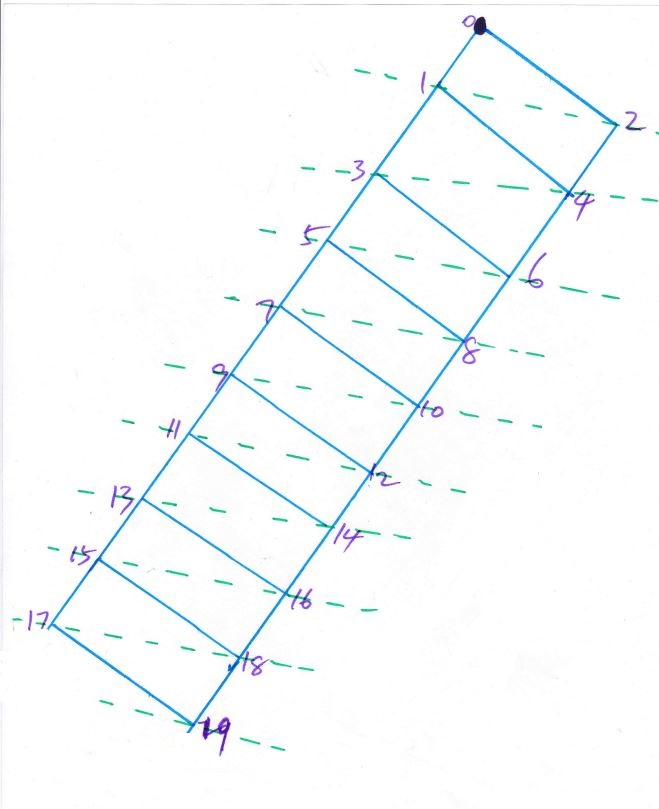
\includegraphics[width=0.7\linewidth]{figure/c210_f}
\caption{2*n $(n = 10)$ regular mesh}
\label{210f}
\end{figure}


\begin{equation}
{
\left[ \begin{array}{ccccccc}
1 & 2 & 2 & \cdots & 2 & 2 & 1\\
1 & -1 & 0 & \cdots& 0 & 0 & 0\\
0 & \sigma-1 & 1 & \cdots & 0 & 0 & 0 \\
0 & \sigma-1 & \sigma & 1 & 0 & \cdots & 0 \\
0 & \sigma-1 & \sigma & \sigma & 1 & 0 & 0 \\
\vdots & \vdots & \vdots  &   \vdots & \ddots & \ddots\\
0 & \sigma-1 & \sigma & \cdots & \sigma & \sigma & 1
\end{array} 
\right ]} \times \left[ \begin{array}{c}
\alpha_{0} \\
\alpha_{1} \\
\alpha_{3} \\
\alpha_{5} \\
\vdots \\
\alpha_{2 \times n - 1}\\
\alpha_{2 \times n + 1}
\end{array} 
\right ] = \left[ \begin{array}{c}
1 \\
0 \\
0 \\
0 \\
\vdots \\
0
\end{array} 
\right ]
\end{equation}

So the Speedup is $$\frac{1}{\alpha_{0}}$$.
\vspace*{50pt}


\vspace*{80pt}
Consider more general case Fig. \ref{38f}.

\begin{figure}[h]
\centering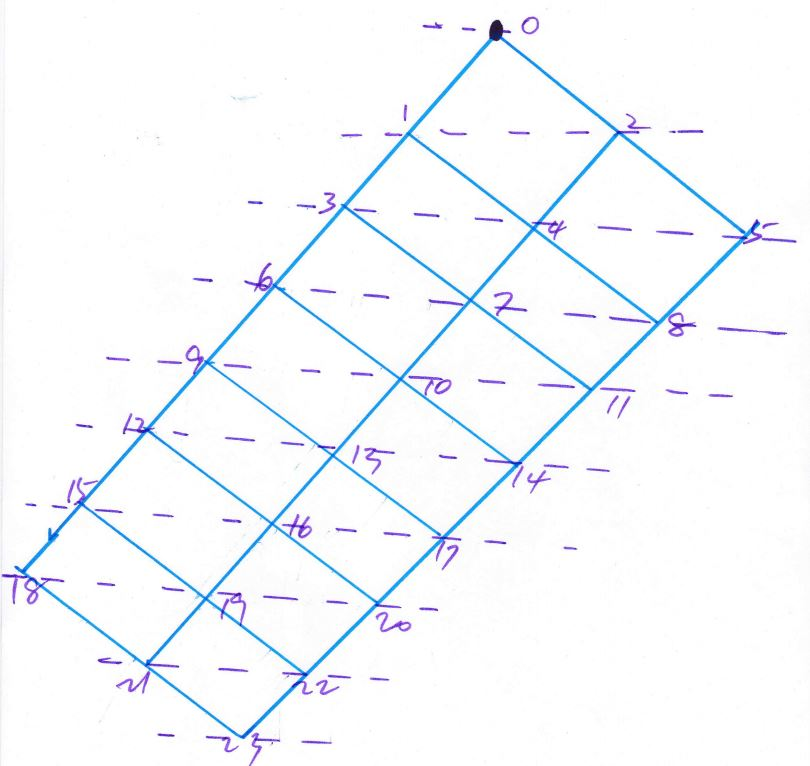
\includegraphics[width=0.7\linewidth]{figure/c38_f}
\caption{3*n $n = 8$ regular mesh}
\label{38f}
\end{figure}

The closed formula groups are presented as following:

\begin{equation}
{
\left[ \begin{array}{cccccccccc}
1 & 2 & 3 & 3 & 3 & 3 & 3 & 3 & 2 & 1\\
1 & -1 & 0 & 0 & 0 & 0 & 0 & 0 & 0 & 0\\
0 & \sigma-1 & 1 & 0 & 0 & 0 & 0 & 0 & 0 & 0 \\
0 & \sigma-1 & \sigma & 1 & 0 & 0 & 0 & 0 & 0 & 0 \\
0 & \sigma-1 & \sigma & \sigma & 1 & 0 & 0 & 0 & 0 & 0\\
0 & \sigma-1 & \sigma & \sigma & \sigma & 1 & 0 & 0 & 0 & 0\\
0 & \sigma-1 & \sigma & \sigma & \sigma & \sigma & 1 & 0 & 0 & 0\\
0 & \sigma-1 & \sigma & \sigma & \sigma & \sigma & \sigma & 1 & 0 & 0\\
0 & \sigma-1 & \sigma & \sigma & \sigma & \sigma & \sigma & \sigma & 1 & 0\\
0 & \sigma-1 & \sigma & \sigma & \sigma & \sigma & \sigma & \sigma & \sigma & 1 \\
\end{array} 
\right ]} \times \left[ \begin{array}{c}
\alpha_{0} \\
\alpha_{1} \\
\alpha_{3} \\
\alpha_{6} \\
\alpha_{9} \\
\alpha_{12}\\
\alpha_{15}\\
\alpha_{18}\\
\alpha_{21}\\
\alpha_{23}
\end{array} 
\right ] = \left[ \begin{array}{c}
1 \\
0 \\
0 \\
0 \\
\vdots \\
0
\end{array} 
\right ]
\end{equation}


\vspace*{50pt}
Consider more general case Fig.\ref{410f} the closed formula groups are presented as following:

\begin{figure}[h]
\centering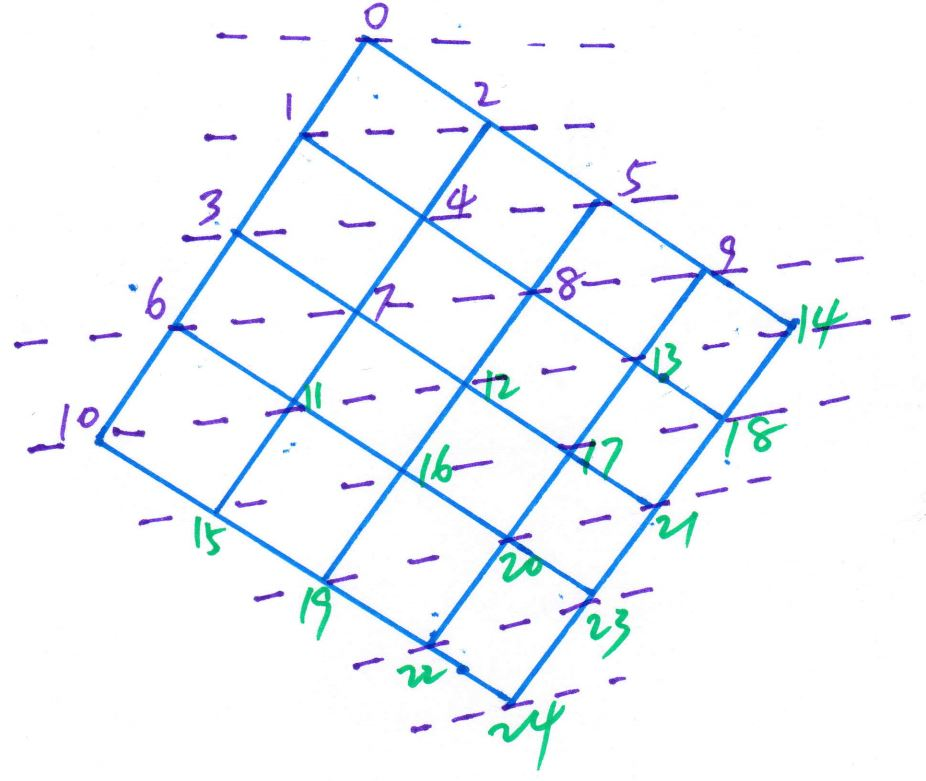
\includegraphics[width=0.7\linewidth]{figure/c410_f}
\caption{m*n $m = 5$, $n = 5$ regular mesh}
\label{410f}
\end{figure}


\begin{equation}
{
\left[ \begin{array}{ccccccccc}
1 & 2 & 3 & 4 & 5 & 4 & 3 & 2 & 1\\
1 & -1 & 0 & 0 & 0 & 0 & 0 & 0& 0\\
0 & \sigma-1 & 1 & 0 & 0 & 0 &0 & 0 & 0 \\
0 & \sigma-1 & \sigma & 1 & 0 & 0 & 0 & 0 & 0 \\
0 & \sigma-1 & \sigma & \sigma & 1 & 0 & 0 & 0 & 0\\
0 & \sigma-1 & \sigma & \sigma & \sigma & 1 & 0& 0 & 0\\
0 & \sigma-1 & \sigma & \sigma & \sigma & \sigma & 1 & 0 & 0\\
0 & \sigma-1 & \sigma & \sigma & \sigma & \sigma & \sigma & 1 & 0\\
0 & \sigma-1 & \sigma & \sigma & \sigma & \sigma & \sigma & \sigma & 1\\
\end{array} 
\right ]} \times \left[ \begin{array}{c}
\alpha_{0} \\
\alpha_{1} \\
\alpha_{3} \\
\alpha_{6} \\
\alpha_{10} \\
\alpha_{15}\\
\alpha_{19}\\
\alpha_{22}\\
\alpha_{24}
\end{array} 
\right ] = \left[ \begin{array}{c}
1 \\
0 \\
0 \\
0 \\
\vdots \\
0
\end{array} 
\right ]
\end{equation}

\vspace*{50pt}

\subsubsection{Load From Boundary Grid Position}
The data injection position lays on the boundary Fig.\ref{e33f} and the regular mesh is 3*3 situation.

\begin{figure}[h]
\centering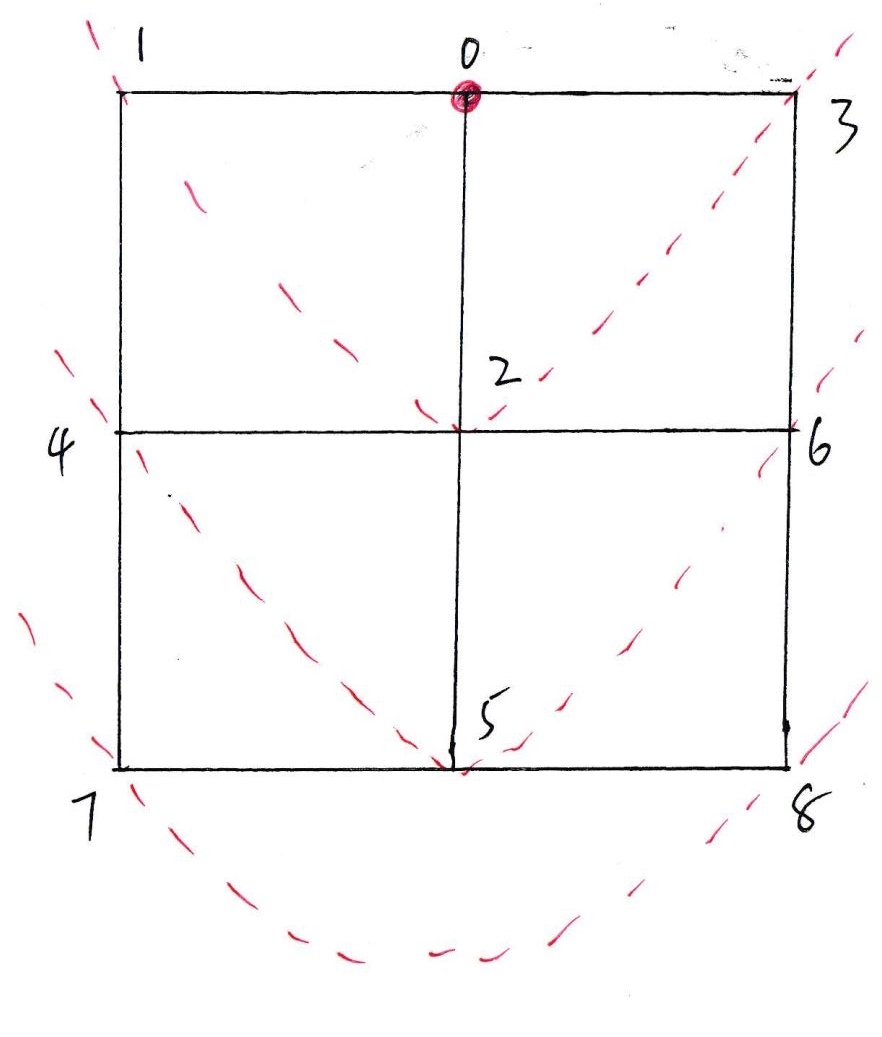
\includegraphics[width= 0.7 \linewidth]{figure/e33_f}
\caption{Data injection position on the boundary of 3*3 regular mesh}
\label{e33f}
\end{figure}

The equation for the boundary data injection condition as follows:

$$\alpha_{0} \omega T_{cp} = T_{f,m}$$ 
$$\alpha_{1} \omega T_{cp} = T_{f,m}$$
$$\alpha_{2} \omega T_{cp} = T_{f,m}$$
$$\alpha_{3} \omega T_{cp} = T_{f,m}$$
$$\alpha_{1}zT_{cm} + \alpha_{4}\omega T_{cp} = T_{f,m}$$
$$\alpha_{2}zT_{cm} + \alpha_{5}\omega T_{cp} = T_{f,m}$$
$$\alpha_{3}zT_{cm} + \alpha_{6}\omega T_{cp} = T_{f,m}$$
$$(\alpha_{1} + \alpha_{4})zT_{cm} + \alpha_{7}\omega T_{cp} = T_{f,m}$$
$$(\alpha_{2} + \alpha_{5})zT_{cm} + \alpha_{8}\omega T_{cp} = T_{f,m}$$

$$\sigma = \frac{zT_{cm}}{\omega T_{cp}}$$

\vspace*{50pt}

\begin{equation}
{
\left[ \begin{array}{cccc}
1 & 3 & 3 & 2\\
1 & -1 & 0 & 0\\
0 & \sigma-1 & 1 & 0\\
0 & \sigma-1 & \sigma & 1
\end{array} 
\right ]} \times \left[ \begin{array}{c}
\alpha_{0} \\
\alpha_{1} \\
\alpha_{4} \\
\alpha_{7}
\end{array} 
\right ] = \left[ \begin{array}{c}
1 \\
0 \\
0 \\
0
\end{array} 
\right ]
\end{equation}

\vspace*{50pt}

\subsubsection{Load From Inner Grid}
\vspace*{5pt}
The data injection position lays on the inner grid position Fig.\ref{i33f} and the regular mesh is 3*3 situation.

\begin{figure}[h]
\centering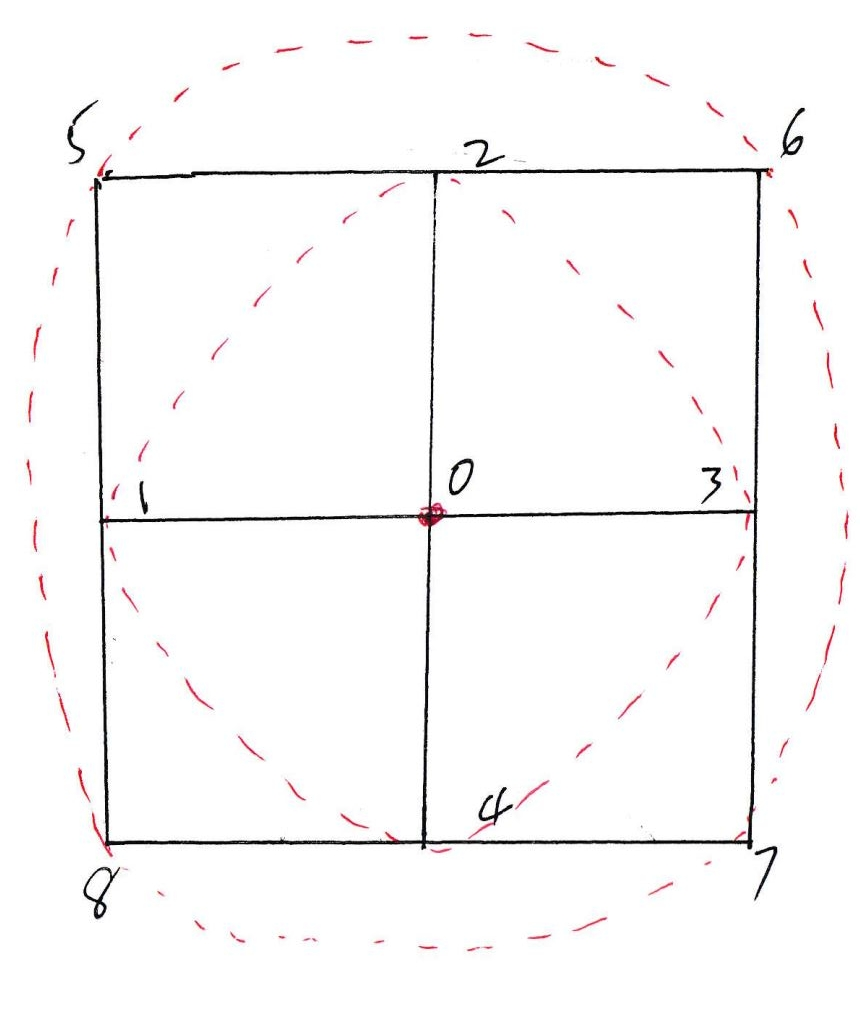
\includegraphics[width= 0.7\linewidth]{figure/i33_f}
\caption{Data injection position on the inner grid position of 3*3 regular mesh}
\label{i33f}
\end{figure}

$$\alpha_{0} \omega T_{cp} = T_{f,m}$$ 
$$\alpha_{1} \omega T_{cp} = T_{f,m}$$
$$\alpha_{2} \omega T_{cp} = T_{f,m}$$
$$\alpha_{3} \omega T_{cp} = T_{f,m}$$
$$\alpha_{4} \omega T_{cp} = T_{f,m}$$
$$\alpha_{1}zT_{cm} + \alpha_{5}\omega T_{cp} = T_{f,m}$$
$$\alpha_{1}zT_{cm} + \alpha_{6}\omega T_{cp} = T_{f,m}$$
$$\alpha_{1}zT_{cm} + \alpha_{7}\omega T_{cp} = T_{f,m}$$
$$\alpha_{1}zT_{cm} + \alpha_{8}\omega T_{cp} = T_{f,m}$$

The equation for the boundary condition as follows:

$$\sigma = \frac{zT_{cm}}{\omega T_{cp}}$$

\vspace*{20pt}

\begin{equation}
{
\left[ \begin{array}{ccc}
1 & 4 & 4 \\
1 & -1 & 0\\
0 & \sigma-1 & 1\\
\end{array} 
\right ]} \times \left[ \begin{array}{c}
\alpha_{0} \\
\alpha_{1} \\
\alpha_{5} \\
\end{array} 
\right ] = \left[ \begin{array}{c}
1 \\
0 \\
0 
\end{array} 
\right ]
\end{equation}


\subsection{General Case}
\begin{equation}
{
\left[ \begin{array}{ccccccc}
1 & m_{1} & m_{2} & \cdots & m_{n-2} & m_{n-1} & m_{n}\\
1 & -1 & 0 & \cdots& 0 & 0 & 0\\
0 & \sigma -1 & 1 & \cdots & 0 & 0 & 0 \\
0 & \sigma -1 & \sigma & 1 & 0 & \cdots & 0 \\
0 & \sigma -1 & \sigma & \sigma & 1 & 0 & 0 \\
\vdots & \vdots & \vdots  &   \vdots & \ddots & \ddots\\
0 & \sigma -1 & \sigma & \cdots & \sigma & \sigma & 1
\end{array} 
\right ]} \times \left[ \begin{array}{c}
\alpha_{l_{0}} \\
\alpha_{l_{1}} \\
\alpha_{l_{2}} \\
\alpha_{l_{3}} \\
\vdots \\
\alpha_{l_{n-1}}\\
\alpha_{l_{n}}
\end{array} 
\right ] = \left[ \begin{array}{c}
1 \\
0 \\
0 \\
0 \\
\vdots \\
0
\end{array} 
\right ]
\end{equation}











\vspace*{5pt}
\subsubsection{Workstation without front-end}

\vspace*{50pt}

We investigate the simple case first and then deduce the more general closed form formula for the regular mesh situation.

\subsection{Load From Corner}
\begin{itemize}

\item 2*2 regular mesh Fig.\ref{22f}
\item 2*3 regular mesh Fig.\ref{23f}
\item 2*n regular mesh,for example $n = 10$ Fig.\ref{210f}
\item 3*n regular mesh,for example $n = 8$ Fig.\ref{38f}
\item m*n regular mesh,for example $m = 5, n = 5$ Fig.\ref{410f}

\end{itemize}

According to Fig.\ref{22f},data injection position comes from corner unit processor.

There are four cores to handle the whole workload in the regular mesh.

$$\alpha_{0} \omega T_{cp} = T_{f,m}$$ 
$$\alpha_{1}zT_{cm} + \alpha_{1} \omega T_{cp} = T_{f,m}$$
$$\alpha_{2}zT_{cm} + \alpha_{2} \omega T_{cp} = T_{f,m}$$
$$(\alpha_{1} + \alpha_{3})zT_{cm} + \alpha_{3}\omega T_{cp} = T_{f,m}$$
$$\sigma = \frac{zT_{cm}}{\omega T_{cp}}$$

\begin{equation}
{
\left[ \begin{array}{ccc}
1 & 2 & 1\\
1 & -(\sigma + 1) & 0\\
1 & -\sigma & -(\sigma + 1)
\end{array} 
\right ]} \times \left[ \begin{array}{c}
\alpha_{0} \\
\alpha_{1} \\
\alpha_{3} 
\end{array} 
\right ] = \left[ \begin{array}{c}
1 \\
0 \\
0 
\end{array} 
\right ]
\end{equation}

\vspace*{50pt}

According to Fig.\ref{23f}, the formula groups are

$$\alpha_{0} \omega T_{cp} = T_{f,m}$$ 
$$\alpha_{1}zT_{cm} + \alpha_{1} \omega T_{cp} = T_{f,m}$$
$$\alpha_{2}zT_{cm} + \alpha_{2} \omega T_{cp} = T_{f,m}$$
$$(\alpha_{1} + \alpha_{3})zT_{cm} + \alpha_{3}\omega T_{cp} = T_{f,m}$$
$$(\alpha_{1} + \alpha_{4})zT_{cm} + \alpha_{4}\omega T_{cp} = T_{f,m}$$
$$(\alpha_{1} + \alpha_{3} + \alpha_{5})zT_{cm} + \alpha_{5}\omega T_{cp} = T_{f,m}$$

\begin{equation}
{
\left[ \begin{array}{cccc}
1 & 2 & 2 & 1\\
1 & -(\sigma + 1) & 0 & 0\\
1 & -\sigma & -(\sigma + 1) & 0\\
1 & -\sigma & -\sigma & -(\sigma + 1)
\end{array} 
\right ]} \times \left[ \begin{array}{c}
\alpha_{0} \\
\alpha_{1} \\
\alpha_{3} \\
\alpha_{5}
\end{array} 
\right ] = \left[ \begin{array}{c}
1 \\
0 \\
0 \\
0
\end{array} 
\right ]
\end{equation}

$$\sigma = \frac{zT_{cm}}{\omega T_{cp}}$$

the speedup ratio is:
$\frac{1}{\alpha_{0}}$

\vspace*{50pt}

According to the 2*n regular mesh, the formula equation group as follows:

$$\alpha_{1}zT_{cm} + \alpha_{1} \omega T_{cp} = T_{f,m}$$
$$\alpha_{2}zT_{cm} + \alpha_{2} \omega T_{cp} = T_{f,m}$$
$$(\alpha_{1} + \alpha_{3})zT_{cm} + \alpha_{3}\omega T_{cp} = T_{f,m}$$
$$(\alpha_{1} + \alpha_{4})zT_{cm} + \alpha_{4}\omega T_{cp} = T_{f,m}$$

$$(\alpha_{1} + \alpha_{3} + \alpha_{5})zT_{cm} + \alpha_{5}\omega T_{cp} = T_{f,m}$$
$$\vdots$$
$$(\alpha_{1} + \alpha_{3} +\cdots + \alpha_{2 \times n + 1})zT_{cm} +\alpha_{2 \times n + 1} \omega T_{cp} = T_{f,m}$$

$$\sigma = \frac{zT_{cm}}{\omega T_{cp}}$$

\begin{equation}
{
\left[ \begin{array}{ccccccc}
1 & 2 & 2 & \cdots & 2 & 2 & 1\\
1 & -(\sigma + 1) & 0 & \cdots& 0 & 0 & 0\\
1 & -\sigma & -(\sigma + 1) & \cdots & 0 & 0 & 0 \\
1 & -\sigma & -\sigma & -(\sigma + 1) & 0 & \cdots & 0 \\
1 & -\sigma & -\sigma & -\sigma & -(\sigma + 1) & 0 & 0 \\
\vdots & \vdots & \vdots  &   \vdots & \ddots & \ddots\\
1 & -\sigma & -\sigma & \cdots & -\sigma & -\sigma & -(\sigma + 1)
\end{array} 
\right ]} \times \left[ \begin{array}{c}
\alpha_{0} \\
\alpha_{1} \\
\alpha_{3} \\
\alpha_{5} \\
\vdots \\
\alpha_{2 \times n - 1}\\
\alpha_{2 \times n + 1}
\end{array} 
\right ] = \left[ \begin{array}{c}
1 \\
0 \\
0 \\
0 \\
\vdots \\
0
\end{array} 
\right ]
\end{equation}

So the Speedup is $$\frac{1}{\alpha_{0}}$$

\vspace*{50pt}

According to the Fig.\ref{38f}, the matrix is:
We use ${\sigma}^{\star}$ to present the $-(\sigma + 1)$

\begin{small}
\begin{equation}
{
\left[ \begin{array}{cccccccccc}
1 & 2 & 3 & 3 & 3 & 3 & 3 & 3 & 2 & 1\\
1 & {\sigma}^{\star} & 0 & 0 & 0 & 0 & 0 & 0 & 0 & 0\\
1 & -\sigma & {\sigma}^{\star} & 0 & 0 & 0 & 0 & 0 & 0 & 0 \\
1 & -\sigma & -\sigma & {\sigma}^{\star} & 0 & 0 & 0 & 0 & 0 & 0 \\
1 & -\sigma & -\sigma & -\sigma & {\sigma}^{\star} & 0 & 0 & 0 & 0 & 0\\
1 & -\sigma & -\sigma & -\sigma & -\sigma & {\sigma}^{\star} & 0 & 0 & 0 & 0\\
1 & -\sigma & -\sigma & -\sigma & -\sigma & -\sigma & {\sigma}^{\star} & 0 & 0 & 0\\
1 & -\sigma & -\sigma & -\sigma & -\sigma & -\sigma & -\sigma & {\sigma}^{\star} & 0 & 0\\
1 & -\sigma & -\sigma & -\sigma & -\sigma & -\sigma & -\sigma & -\sigma & {\sigma}^{\star} & 0\\
1 & -\sigma & -\sigma & -\sigma & -\sigma & -\sigma & -\sigma & -\sigma & -\sigma & -{\sigma}^{\star} \\
\end{array} 
\right ]} \times \left[ \begin{array}{c}
\alpha_{0} \\
\alpha_{1} \\
\alpha_{3} \\
\alpha_{6} \\
\alpha_{9} \\
\alpha_{12}\\
\alpha_{15}\\
\alpha_{18}\\
\alpha_{21}\\
\alpha_{23}
\end{array} 
\right ] = \left[ \begin{array}{c}
1 \\
0 \\
0 \\
0 \\
\vdots \\
0
\end{array} 
\right ]
\end{equation}
\end{small}


\vspace*{50pt}
According to the Fig. \ref{410f}, the formula groups as follows:
We use ${\sigma}^{\star}$ to present the $-(\sigma + 1)$

\begin{equation}
{
\left[ \begin{array}{ccccccccc}
1 & 2 & 3 & 4 & 5 & 4 & 3 & 2 & 1\\
1 & {\sigma}^{\star} & 0 & 0 & 0 & 0 & 0 & 0 & 0\\
1 & -\sigma & {\sigma}^{\star} & 0 & 0 & 0 & 0& 0 & 0 \\
1 & -\sigma & -\sigma & {\sigma}^{\star} & 0 &0 & 0 & 0 & 0 \\
1 & -\sigma & -\sigma & -\sigma & {\sigma}^{\star} & 0 & 0 & 0 & 0\\
1 & -\sigma & -\sigma & -\sigma & -\sigma & {\sigma}^{\star} & 0 & 0 & 0\\
1 & -\sigma & -\sigma & -\sigma & -\sigma & -\sigma & {\sigma}^{\star} & 0 & 0\\
1 & -\sigma & -\sigma & -\sigma & -\sigma & -\sigma & -\sigma & {\sigma}^{\star} &0\\
1 & -\sigma & -\sigma & -\sigma & -\sigma & -\sigma & -\sigma & -\sigma & {\sigma}^{\star}\\
\end{array} 
\right ]} \times \left[ \begin{array}{c}
\alpha_{0} \\
\alpha_{1} \\
\alpha_{3} \\
\alpha_{6} \\
\alpha_{10} \\
\alpha_{15}\\
\alpha_{19}\\
\alpha_{22}\\
\alpha_{24}
\end{array} 
\right ] = \left[ \begin{array}{c}
1 \\
0 \\
0 \\
0 \\
\vdots \\
0
\end{array} 
\right ]
\end{equation}


\vspace*{50pt}
\subsubsection{Load From Boundary Grid Position}
The data injection position lays on the boundary Fig.\ref{e33f} and the regular mesh is 3*3 situation.

$$\alpha_{0} \omega T_{cp} = T_{f,m}$$ 
$$\alpha_{1}zT_{cm} + \alpha_{1} \omega T_{cp} = T_{f,m}$$
$$\alpha_{2}zT_{cm} + \alpha_{2} \omega T_{cp} = T_{f,m}$$
$$\alpha_{3}zT_{cm} + \alpha_{3} \omega T_{cp} = T_{f,m}$$
$$(\alpha_{1} + \alpha_{4})zT_{cm} + \alpha_{4}\omega T_{cp} = T_{f,m}$$
$$(\alpha_{2} + \alpha_{5})zT_{cm} + \alpha_{5}\omega T_{cp} = T_{f,m}$$
$$(\alpha_{3} + \alpha_{6})zT_{cm} + \alpha_{6}\omega T_{cp} = T_{f,m}$$
$$(\alpha_{1} + \alpha_{4} +\alpha_{7})zT_{cm} + \alpha_{7}\omega T_{cp} = T_{f,m}$$
$$(\alpha_{1} + \alpha_{4} +\alpha_{8})zT_{cm} + \alpha_{8}\omega T_{cp} = T_{f,m}$$

The equation for the boundary condition as follows:

$$\sigma = \frac{zT_{cm}}{\omega T_{cp}}$$
\begin{equation}
{
\left[ \begin{array}{cccc}
1 & 3 & 3 & 2\\
1 & -(\sigma + 1) & 0 & 0\\
1 & -\sigma & -(\sigma + 1) & 0\\
1 & -\sigma & -\sigma & -(\sigma + 1)
\end{array} 
\right ]} \times \left[ \begin{array}{c}
\alpha_{0} \\
\alpha_{1} \\
\alpha_{4} \\
\alpha_{7}
\end{array} 
\right ] = \left[ \begin{array}{c}
1 \\
0 \\
0 \\
0
\end{array} 
\right ]
\end{equation}



\vspace*{50pt}
\subsubsection{Load From Inner Grid}
The data injection position lays on the inner grid position Fig.\ref{i33f} and the regular mesh is 3*3 situation.

$$\alpha_{0} \omega T_{cp} = T_{f,m}$$ 
$$\alpha_{1}zT_{cm} + \alpha_{1} \omega T_{cp} = T_{f,m}$$
$$\alpha_{2}zT_{cm} + \alpha_{2} \omega T_{cp} = T_{f,m}$$
$$\alpha_{3}zT_{cm} + \alpha_{3} \omega T_{cp} = T_{f,m}$$
$$\alpha_{4}zT_{cm} + \alpha_{4} \omega T_{cp} = T_{f,m}$$
$$(\alpha_{1} + \alpha_{5})zT_{cm} + \alpha_{5}\omega T_{cp} = T_{f,m}$$
$$(\alpha_{2} + \alpha_{6})zT_{cm} + \alpha_{6}\omega T_{cp} = T_{f,m}$$
$$(\alpha_{3} + \alpha_{7})zT_{cm} + \alpha_{7}\omega T_{cp} = T_{f,m}$$
$$(\alpha_{4} + \alpha_{8})zT_{cm} + \alpha_{8}\omega T_{cp} = T_{f,m}$$

The equation for the boundary data injection condition as follows:

$$\sigma = \frac{zT_{cm}}{\omega T_{cp}}$$

\begin{equation}
{
\left[ \begin{array}{ccc}
1 & 4 & 4 \\
1 & -(\sigma + 1) & 0\\
1 & -\sigma & -(\sigma + 1)\\
\end{array} 
\right ]} \times \left[ \begin{array}{c}
\alpha_{0} \\
\alpha_{1} \\
\alpha_{5} \\
\end{array} 
\right ] = \left[ \begin{array}{c}
1 \\
0 \\
0 
\end{array} 
\right ]
\end{equation}
\vspace*{50pt}


\subsubsection{General Case}
\begin{equation}
{
\left[ \begin{array}{ccccccc}
1 & m_{1} & m_{2} & \cdots & m_{n-2} & m_{n-1} & m_{n}\\
1 & -(\sigma + 1) & 0 & \cdots& 0 & 0 & 0\\
1 & -\sigma & -(\sigma + 1) & \cdots & 0 & 0 & 0 \\
1 & -\sigma & -\sigma & -(\sigma + 1) & 0 & \cdots & 0 \\
1 & -\sigma & -\sigma & -\sigma & -(\sigma + 1) & 0 & 0 \\
\vdots & \vdots & \vdots  &   \vdots & \ddots & \ddots\\
1 & -\sigma & -\sigma & \cdots & -\sigma & -\sigma & -(\sigma + 1)
\end{array} 
\right ]} \times \left[ \begin{array}{c}
\alpha_{l_{0}} \\
\alpha_{l_{1}} \\
\alpha_{l_{2}} \\
\alpha_{l_{3}} \\
\vdots \\
\alpha_{l_{n-1}}\\
\alpha_{l_{n}}
\end{array} 
\right ] = \left[ \begin{array}{c}
1 \\
0 \\
0 \\
0 \\
\vdots \\
0
\end{array} 
\right ]
\end{equation}
\vspace*{5pt}
\subsubsection{Speedup Result between front-end schema and without front-end schema}
\begin{figure}[h]
\centering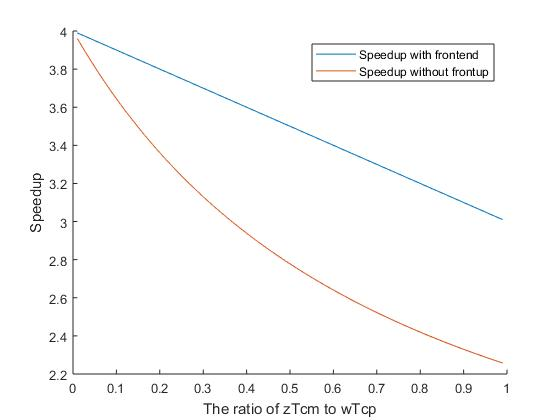
\includegraphics[width=0.7\linewidth]{figure/c22}
\caption{Speedup vs $\sigma$ value in 2*2 regular mesh}
\label{22}
\end{figure}

\begin{figure}[h]
\centering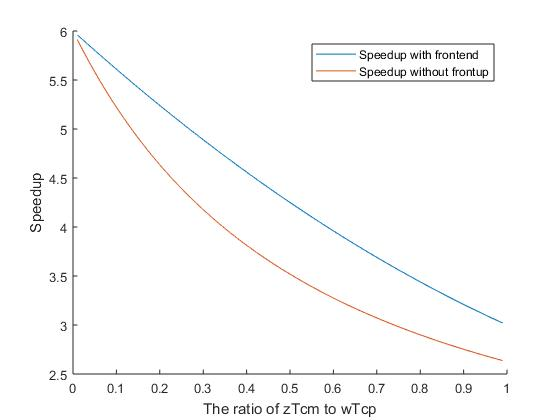
\includegraphics[width=0.7\linewidth]{figure/c23}
\caption{Speedup vs $\sigma$ value in 2*3 regular mesh}
\label{23}
\end{figure}

\begin{figure}[h]
\centering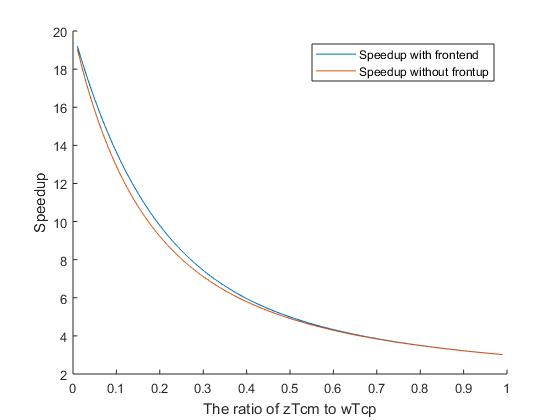
\includegraphics[width=0.7\linewidth]{figure/c210}
\caption{Speedup vs $\sigma$ value in 2*10 regular mesh}
\label{210}
\end{figure}

\begin{figure}[h]
\centering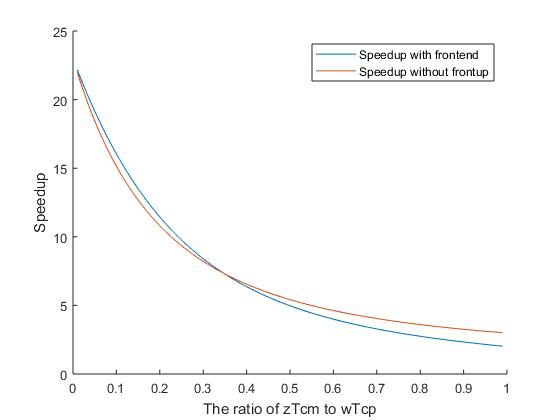
\includegraphics[width=0.7\linewidth]{figure/c38}
\caption{Speedup vs $\sigma$ value in 3*8 regular mesh}
\label{38}
\end{figure}

\begin{figure}[h]
\centering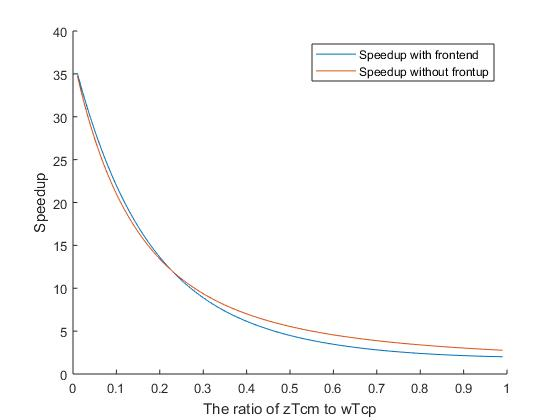
\includegraphics[width=0.7\linewidth]{figure/c410}
\caption{Speedup vs $\sigma$ value in 4*10 regular mesh}
\label{410}
\end{figure}




